\chapter{Inflationary Cosmology}
\label{chp:cos}

\section{Introduction}
\label{sec:cos:intro}

This chapter reviews the key concepts of inflationary cosmology, and mostly serves to establish notation.
For further detail, excellent references can be found in~\cite{Wald},~\cite{Hobson} \&~\cite{Dodelson}.

\section{Einstein's gravity}
\label{sec:cos:einsteins_gravity}
\begin{quote}
  {\em Spacetime tells matter how to move;\\ matter tells spacetime how to curve.}\hfill
  --- \johnwheeler{}
\end{quote}

Einstein's theory of general relativity accounts for gravity by removing it as a fundamental force and considering gravitation as a property of spacetime itself. Objects and fields still interact with one another on a spacetime background via the usual forces (electromagnetic, strong and weak nuclear forces). The background spacetime can be thought of as curved, and the perceived effect of gravitation is due to objects moving on straight paths in a curved spacetime. Finally, the curvature (and thus gravitation) is generated by the matter content of the spacetime.

The formalism of Einstein's gravity can be effectively summarised using the Einstein-Hilbert action. An action \(S\) is written as a general relativistic integral over a Lagrangian density \(\mathcal{L}\):
\begin{equation}
  S = \int\d[4]{x} \sqrt{|g|} \mathcal{L}.
  \label{eqn:cos:generic_lagrangian}
\end{equation}
where the factor of \(\sqrt{g}\), \(g=\left|\det\left( g_{\mu\nu} \right)\right|\) ensures a relativistic volume element for integration.
We typically decompose the Lagrangian \(\mathcal{L}\) into a gravitational and matter part:
\begin{align}
  \mathcal{L} &= \mathcal{L}_G + \mathcal{L}_M,
  \label{eqn:cos:decomp}\\
  \mathcal{L}_G &= \frac{1}{2} \m^2 R,
  \label{eqn:cos:L_grav}
\end{align}
where \(R\) is the Ricci scalar and \(\mathcal{L}_M\) is the portion of the Lagrangian pertaining to the material content of spacetime. Requiring that the action~\eqref{eqn:cos:generic_lagrangian} is extremal (\(\delta S = 0\)) yields Einstein's equations:
\begin{equation}
  G_{\mu\nu} = \frac{1}{\m^2}T_{\mu\nu},
  \label{eqn:cos:einsteins_equations}
\end{equation}
where:
\begin{equation}
  T_{\mu\nu} = \frac{-2}{\sqrt{\abs{g}}}\frac{\delta}{\delta g^{\mu\nu}}\left( \sqrt{\abs{g}} \mathcal{L}_M \right),
  \label{eqn:cos:SET_fundamantal}
\end{equation}
is the stress energy tensor, and:
\begin{equation}
  G_{\mu\nu} = R_{\mu\nu} - \frac{1}{2}g_{\mu\nu} R,
  \label{eqn:cos:einstein_tensor}
\end{equation}
is the Einstein tensor. The symmetries of the Einstein tensor~\eqref{eqn:cos:einstein_tensor} mean that there are in fact only six independent equations in~\eqref{eqn:cos:einsteins_equations}. Further, the fact that \(\nabla^\mu G_{\mu\nu}=0\) means that the stress energy tensor is conserved:
\begin{equation}
  \nabla_\mu {T^{\mu}}_{\nu} = 0.
  \label{eqn:cos:SET_conservation}
\end{equation}
This conservation equation can provide a fast means for deriving alternative rearrangements of the Einstein equations.\footnote{Historical note: Einstein in fact derived this argument in reverse. He defined the Einstein tensor~\protect\eqref{eqn:cos:einstein_tensor} by adjusting the Ricci tensor so that the stress energy tensor is conserved by construction. In the more modern approach presented here, the definition of the Einstein tensor arises naturally from variational principles.}

\section{The smooth, expanding universe}
On the largest scales, we observe the universe to be spatially {\em homogeneous\/} and {\em isotropic}. This justifies the philosophical {\em cosmological principle}, that the universe should look the same wherever you are, and that no place in the universe is special. 

In this section, we examine the consequences that these observations have within the context of general relativity, by considering the solutions to the Einstein equations~\eqref{eqn:cos:einsteins_equations}.

\subsection{Metric}
\begin{table}[tp]
  \centering
  \begin{tabular}{ll}
 \toprule
  Symbol & Definition \\
 \midrule
 \midrule
  $t$ & cosmic time \\
  $X$ & Spatial coordinate \\
  $\chi$ & Comoving radial coordinate \\
  $\theta$ & polar angle \\
  $\phi$ & azimuthal angle \\
  $\Omega$ & solid angle \\
  $a$ & cosmic scale factor \\
  $k=+1$ & closed universe \\
  $k=0$ & flat universe \\
  $k=-1$ & open universe \\
 \bottomrule
\end{tabular}

\caption{Definitions of terms in the FRW metric.}\label{tab:cos:metric}
\end{table}

In any general relativistic analysis, it is helpful to restrict the form of the metric via the symmetries of the problem.
Under the assumption of the cosmological principle, the metric may always be written in the Friedmann-Robertson-Walker form:
\begin{equation}
  \d{s}^2 = \d{t}^2 - a{(t)}^2 \d{X}^2,
  \label{eqn:cos:FRW_metric}
\end{equation}
where:
\begin{align}
  \d{X}^2 &= \d{\chi}^2 + S_k^2{(\chi)} \d{\Omega}
  \label{eqn:cos:space_element}\\
  \d{\Omega} &= \d{\theta}^2 + \sin^2\theta \d{\phi}^2,
  \label{eqn:cos:angle_element}\\
  S_k^2(\chi) &=
  \left\{
  \begin{array}{rl}
    \sin^2\chi &: k>0 \\
    \chi^2 &: k=0 \\
    \sinh^2\chi &: k<0. \\
  \end{array}
  \right.\label{eqn:cos:S_def}
\end{align}
The definitions of these terms can be found in Table~\ref{tab:cos:metric}. 

The form of the metric~\eqref{eqn:cos:FRW_metric} is close to Minkowski. Spatial slices at constant \(t\) are spaces with constant curvature, which may be positive, negative or zero (corresponding to a closed, open or flat universe). The time dependency of the spatial part is a scaling by a scale factor \(a(t)\). As cosmic time \(t\) increases, \(a(t)\) evolves, causing the spatial slice to expand or contract (Figure~\ref{fig:cos:comoving_vs_physical}). 



\begin{figure}[tp]
  \centering
  \tikzsetnextfilename{comoving}
  \includegraphics[width=\textwidth]{chapters/inflationary_cosmology/plots/comoving.tikz}
  \caption{The expansion of the universe. As the universe evolves with time, the scale factor \(a(t)\) changes. The scale factor \(a(t)\) connects {\em comoving coordinates}, \(X\) with {\em physical coordinates}, \(x=a(t)X\). Comoving variables can be thought of as a time-independent grid, which expands with the universe, physical variables are what observers would measure as distances. Hence, in an expanding universe, the physical distance between observers (dots in the diagram above) appears to increase over time, whilst their comoving distance remains the same.}\label{fig:cos:comoving_vs_physical}
\end{figure}


\subsection{Dynamics}
In order to obtain the equations governing \(a(t)\) and thus the dynamics of the universe, we must make some assumptions about the universe's contents. For a smooth universe, one may model its contents as a collection of non-interacting, comoving, uniform, perfect fluids. A perfect fluid in thermodynamic equilibrium has stress-energy tensor:
\begin{equation}
  T^{\mu\nu} = (P+\rho)u^{\mu}u^{\nu} - P g^{\mu\nu} + \Sigma^{\mu\nu},
  \label{eqn:cos:SET_perfect_fluid}
\end{equation}
where \(\rho\) is the energy density, \(P\) is the pressure, \(u^\mu\) is the four velocity of the fluid, and \(\Sigma^{\mu\nu}\) is a traceless, symmetric, anisotropic stress term. In accordance with the cosmological principle, we shall assume that in the comoving frame the fluid is stationary \(u^\mu = [1,\bzero]\), and uniform \(\rho=\rho(t),P=P(t)\), with no anisotropy \(\Sigma=0\).  

Applying the metric~\eqref{eqn:cos:FRW_metric} to the Einstein equations~\eqref{eqn:cos:einsteins_equations}, with the stress-energy tensor~\eqref{eqn:cos:SET_perfect_fluid} one finds:
\begin{align}
  \dot{H}+H^2 &= 
  -\frac{1}{6\m^2}\left( \rho + 3P\right), 
  \label{eqn:cos:Raychaudhuri}
  \\
  H^2 &= 
  \frac{1}{3\m^2}\rho - \frac{k}{a^2}, 
  \label{eqn:cos:Friedmann}
\end{align}
%
where \(H=\dot{a}/a\) is the Hubble parameter and a dot denotes differentiation with respect to cosmic time, \(\dot{f}\equiv \d{f}/\d{t}\). These are termed the {\em acceleration\/} and {\em Friedmann\/} equations respectively, and implicitly govern the dynamics of the scale factor \(a(t)\). It should be noted that these equations are not complete, as additionally one requires an equation of state linking \(\rho\) and \(P\).

\subsection{Basic solutions}
A reasonable model for the universe we observe today is to treat the matter as a multi-component fluid, with each component with its own equation of state:
\begin{equation}
  \rho = \sum_i \rho_i, \qquad P = \sum_i P_i, \qquad P_i = w_i \rho_i,
  \label{eqn:cos:multi_component}
\end{equation}
where \(w_i\) is the equation of state parameter. In our universe, we observe matter \((w=0)\), radiation \((w=\frac{1}{3})\) and dark energy \((w\approx
-1)\). We can also notationally model the curvature's scale-factor contribution of \(-\frac{k}{a^2}\) as a cosmological fluid with \(w=-\frac{1}{3}\). Applying these equations of states, equations~\eqref{eqn:cos:Raychaudhuri} and~\eqref{eqn:cos:Friedmann} may be re-cast as an equation purely in \(a\):
\begin{equation}
  {\left( \frac{H}{H_0} \right)}^2 \equiv 
  \frac{1}{H_0^2}{\left( \frac{\dot{a}}{a} \right)}^2 =
  \Omega^\text{(rad)}_0 a^{-4} +
  \Omega^\text{(mat)}_0 a^{-3} + 
  \Omega^\text{(curv)}_0 a^{-2} +
  \Omega^\text{(de)}_0,
  \label{eqn:cos:expansion_history}
\end{equation}
where the present-day \((t=t_0)\) scale factor is chosen to be unity \((a(t_0)=1)\), quantities subscripted with \(0\) indicate the present-day  value of the parameter, and the density parameter \(\Omega\) is defined as:
\begin{equation}
  \Omega = \frac{\rho}{\rho_\mathrm{c}}, \qquad \rho_\mathrm{c} = {3\m^2H^2},
  \label{eqn:cos:omega_def}
\end{equation}
which measures the fraction of the critical density \(\rho_c\) taken up by a given component. Equation~\eqref{eqn:cos:expansion_history} cannot be analytically solved in general, but if one assumes that one component is dominant, and the rest negligible, then one recovers the solution:
\begin{equation}
  a  \propto
  \left\{
  \begin{array}{ll}
    t^{2/3(w+1)} &: w\ne-1\\
    e^{H_0 t} &: w=-1.\\
  \end{array}
  \right.
\end{equation}
We can see immediately that in a universe dominated by dark energy \({(w\approx-1)}\) the expansion is exponential, and in one dominated by radiation \({(w=1/3)}\), that \({a\propto t^{1/2}}\), which is a slower expansion than one dominated by matter \({a\propto t^{2/3}}\). For our universe, we observe that it is approximately flat \({\Omega_0^{\text{(curv)}}\approx0}\), and that matter today is of the same order of magnitude as dark energy but vastly outweighs radiation \({\Omega_0^{\text{(de)}} \approx \Omega_0^{\text{(mat)}} \gg \Omega_0^{\text{(rad)}}}\). We thus expect an expansion history of the form shown in Figure~\ref{fig:cos:expansion_history}.

\begin{figure}[tp]
  \centering
  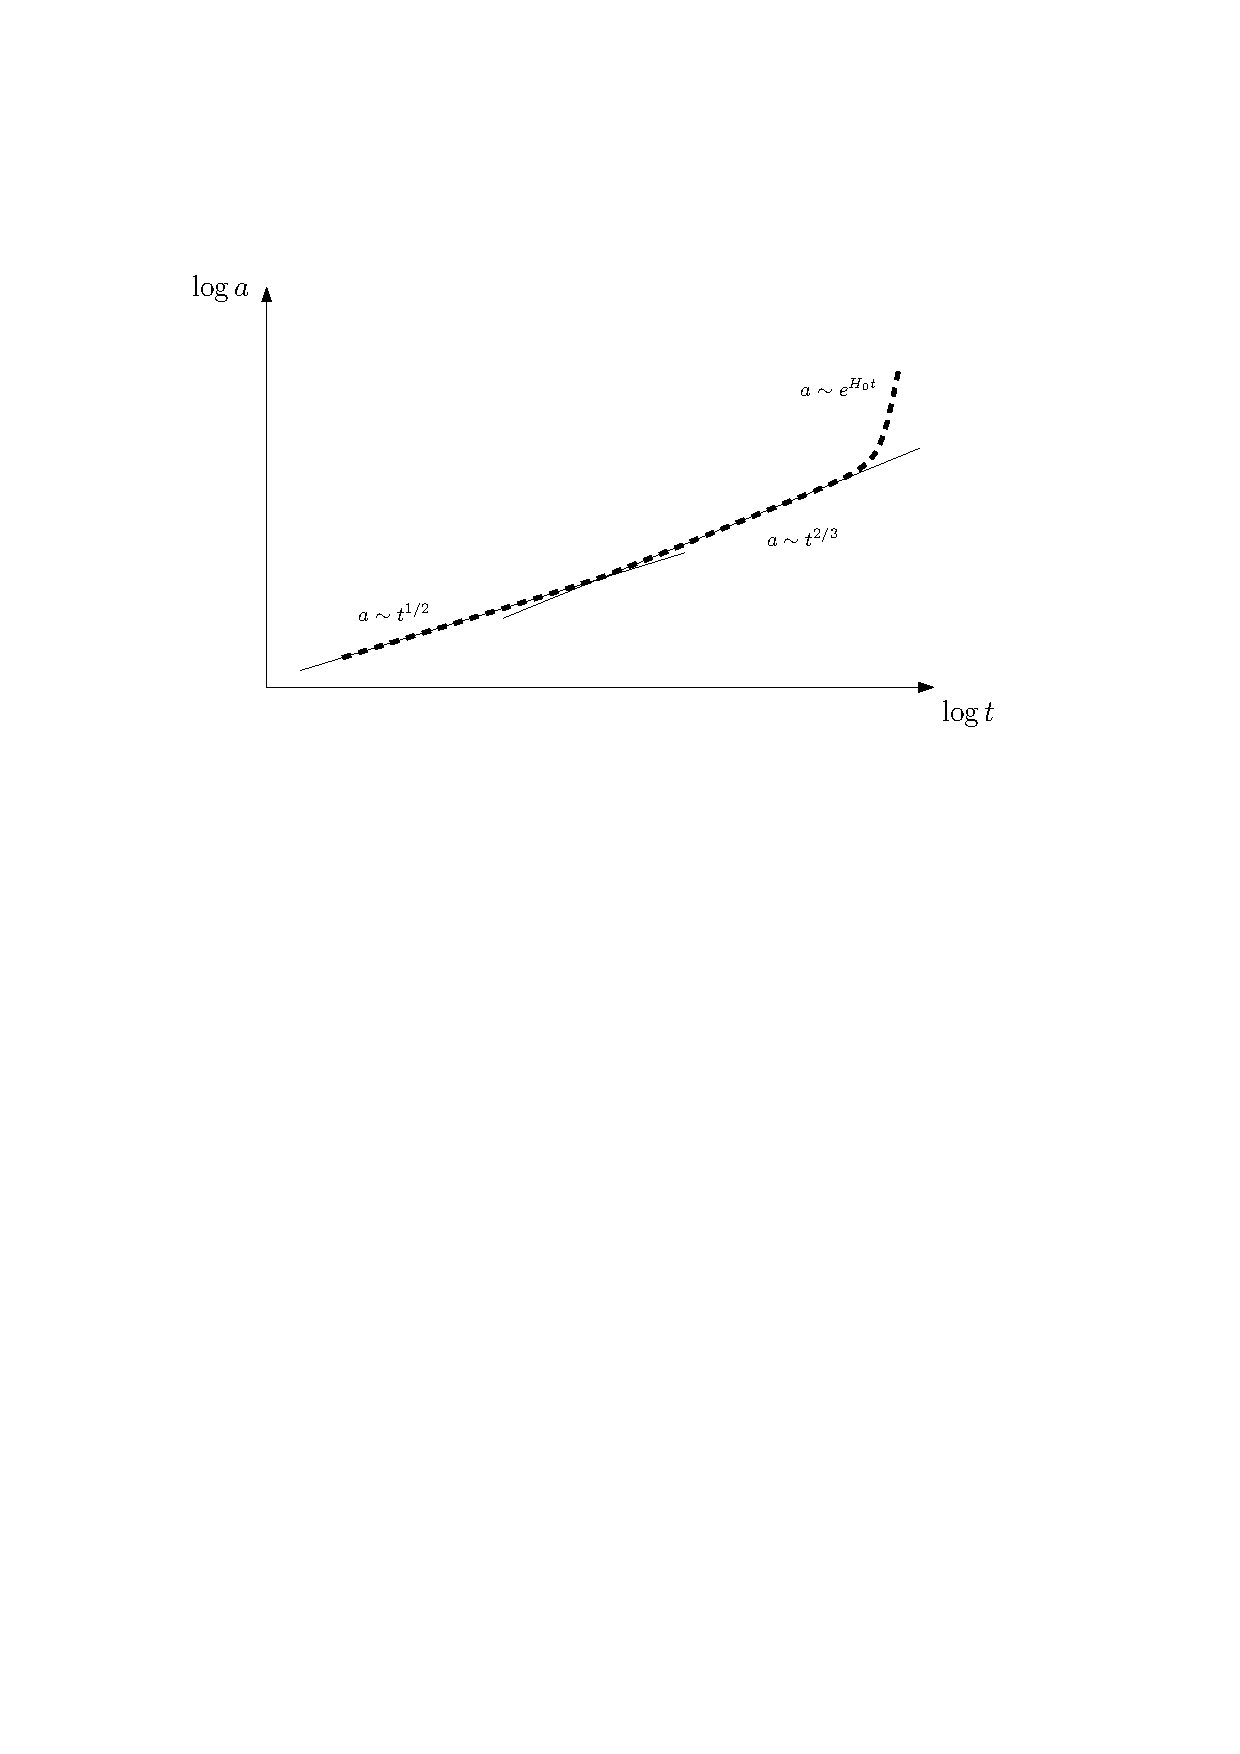
\includegraphics[width=\textwidth]{chapters/inflationary_cosmology/figures/expansion_history}
  \caption{The approximate expansion history of our universe. Initially, the universe is dominated by radiation \(a\sim t^{1/2}\). As the universe expands, the photons lose energy as their wavelengths are stretched.  Thus, the universe transitions to a matter dominated \(a\sim t^{2/3}\) regime. Finally, the dark energy of the universe overtakes the matter content, causing an exponential expansion \(a\sim e^{H_0 t}\).}\label{fig:cos:expansion_history}
\end{figure}


\section{Conformal time and redshift}
\subsection{Redshift \(z\)}
The expansion of the universe causes the wavelengths of photons to increase: Photons have a four-momentum proportional to their wavevector \(p^\mu \propto k^\mu\). Since the FRW metric has no explicit \(\chi\)-dependence for radially travelling photons, \(p_\chi\) is conserved: \(p_\chi(t_1) = p_\chi(t_2)\). Using the metric to raise the indices, one finds that \(p^\chi(t_2){a(t_2)}^2=p^\chi(t_1){a(t_1)}^2\). Identifying the physical momentum \({a p^\chi \propto k^r \propto \lambda^{-1}}\) where \(\lambda\) is the wavelength of the photon, one finds:
\begin{equation}
  \frac{\lambda_2}{\lambda_1} = \frac{a_2}{a_1},
\end{equation}
and thus the wavelengths of photons increase with the expansion of the universe. Physically, the stretching of spacetime stretches the wavelengths of photons.
The redshift \(z\) of the photon from some early time \(t_1\), relative to the current epoch \(t_0\), is defined as usual as:
\begin{equation}
  z = \frac{\lambda_0-\lambda_1}{\lambda_1},
\end{equation}
which gives a relation between the redshift of a photon and the scale factor:
\begin{equation}
  a = \frac{1}{1+z}.
\end{equation}
Since redshift is a physically observable quantity, it provides a cosmology-independent measure of the epoch of the universe (Table~\ref{tab:cos:universe_timeline}).
\begin{table}[tp]
  \centering
  \begin{tabular}{ll}
 \toprule
  Epoch & Redshift \\
 \midrule
 \midrule
 Matter-radiation equality &
 $z\sim3400$
 \\
 Recombination &
 $z\sim1089$
 \\
 Dark ages &
 $20<z<1089$
 \\
 First stars &
 $z\sim20$
 \\
 Reionisation &
 $6<z<20$
 \\
 Dark energy-matter equality &
 $z=0.4$
 \\
 Now &
 $z=0$
 \\
 \bottomrule
\end{tabular}

\caption{Recent history of the universe. As redshift is a directly observable quantity, it provides a natural measure of cosmic epoch.}\label{tab:cos:universe_timeline}
\end{table}

\subsection{Conformal time \(\eta\)}

It is convenient to define conformal time as:
\begin{equation}
  \eta = \int \frac{\d{t}}{a},
  \label{eqn:cos:conformal_time}
\end{equation}
so that the line element becomes:
\begin{equation}          
  \d{s}^2 = {a(\eta)}^2\left( \d{\eta}^2 - \d{X}^2 \right).
  \label{eqn:cos:flat_FRW}
\end{equation}
This is often analytically useful, as it demonstrates the metric is conformally equivalent to Minkowski space\footnote{Hence the name ``conformal time''.}. Physically conformal time corresponds to a temporal coordinate in which photons appear as if they were in flat space: If we consider (without loss of generality) radially travelling photons \(\d{\Omega}=0\) the line element is:
\begin{equation}          
  \d{s}^2 = a(\eta)\left( \d{\eta}^2 - \d{\chi}^2 \right).
  \label{eqn:cos:flat_FRW_radial}
\end{equation}
We have thus removed all the complexities of curvature and comoving coordinates. Since photons have a null trajectory, \(ds^2=0\Rightarrow \d{\eta} = \pm \d{\chi}\), and therefore  travel in straight lines on spacetime diagrams with \(\eta\) and \(\chi\) as axes. This considerably simplifies most pictures.\footnote{For example, later in the chapter Figures~\protect\ref{fig:cos:horizon_problem} \&~\protect\ref{fig:cos:horizon_problem_resolved} both use this construction.}  It can therefore be thought of as a ``comoving'' time, in analogy with comoving spatial coordinates.\footnote{Alternatively, conformal time is the time measured by a small light clock that expands comovingly with the universe.}

\section{The cosmic microwave background}

\begin{figure}[tp]
  \centering
  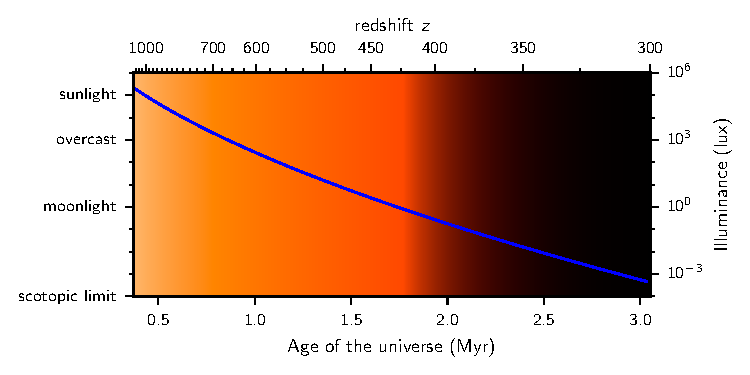
\includegraphics[width=\textwidth]{chapters/inflationary_cosmology/figures/cmb_colour}
  \caption{The colour and illuminance of the radiation background, as a function of cosmic history. As the universe ages, the initially optical background gradually redshifts all the way down to the microwaves that are observed today. This plot shows the colour and the perceived irradiance (illuminance) that the CMB would appear to be in the first few million years after last scattering. For example, for an observer (un)fortunate enough to be born \(500,000\) years after the big bang, the universe would still be bathed in orange light from all directions.}\label{fig:cos:cmb_colour}
\end{figure}

As we turn telescopes on objects further away from earth, we begin to look appreciably back in time. The radiation from these objects has taken so long to reach us that we can observe the universe in a much younger state than it is now. The furthest galaxies imaged by the Hubble space telescope are more than 13 billion years old. Many of these objects are so far away that they have redshifted out of the visible spectrum and into the infra-red. If we look beyond, we enter the dark ages of the universe, before the first stars had turned on. This would appear to be the end of the observational story.

However, from behind the dark ages, there is a background of microwaves. These would originally have been emitted as optical light, but have redshifted all the way down to the microwave end of the spectrum (Figure~\ref{fig:cos:cmb_colour}). This uniform backdrop of radiation is our direct image of the universe as it was at redshift \(z\sim1000\), when the universe was a mere \(380,000\) years old.

Since its first (accidental) detection in 1964 by~\cite{PenziasWilson}, a succession of microwave telescopes, both on the ground and in space, have sharpened our image of this (Figure~\ref{fig:cos:satellites}).
The cosmic microwave background (CMB) is found to be:
\begin{enumerate}
  \item A near-perfect blackbody spectrum, with \(T_0=2.7254(5)\)K.
  \item Isotropic to one part in \(10^{5}\). The minute anisotropies have non-trivial power spectrum, and contain a wealth of cosmological information.
\end{enumerate}

\begin{figure}[tp]
  \centering
  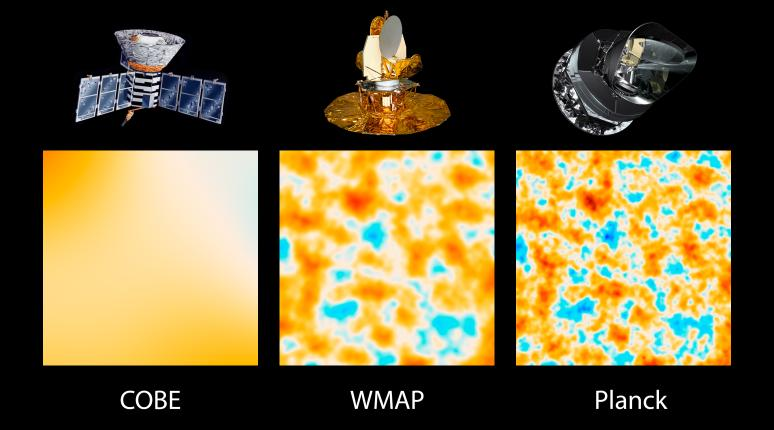
\includegraphics[width=\textwidth]{chapters/inflationary_cosmology/figures/satellites}
  \caption{Microwave satellite images of the minute CMB anisotropies. COBE ran from 1989--1993, WMAP from 2001--2010 and Planck from 2009--2013.}\label{fig:cos:satellites}
\end{figure}

\section{Problems in the CMB}
\subsection{Flatness problem}
The degree to which the universe is not flat can be measured by re-writing the Friedmann equation~\eqref{eqn:cos:Friedmann} in terms of \(\Omega\) as in~\eqref{eqn:cos:omega_def}:
\begin{equation}
  1-\Omega = -\frac{k}{{(aH)}^2} \equiv \Omega_k.
  \label{eqn:cos:friedmann_omega}
\end{equation}
In terms of these kind of variables, the acceleration equation~\eqref{eqn:cos:Raychaudhuri} is:
\begin{equation}
  \frac{\d{\log aH}}{\d{\log a} } = -\frac{1}{2}\Omega(1+3w),
  \label{eqn:cos:raychaudhuri_omega}
\end{equation}
where here \(w=P/\rho\) is not necessarily constant.
Taking absolute logarithms of~\eqref{eqn:cos:friedmann_omega}, differentiating and applying~\eqref{eqn:cos:raychaudhuri_omega} yields:
\begin{equation}
  \frac{\d{\log |\Omega-1|}}{\d{\log a} } = \Omega(1+3w).
  \label{eqn:cos:instability}
\end{equation}
One can see from this that a flat universe \((\Omega=1)\) is an unstable point of equilibrium of these equations, provided that \(1+3w>0\). For both matter (\({w=0}\)) and radiation (\({w=\frac{1}{3}}\)), the universe is rapidly driven away from flatness as the universe expands. This is natural, as the effect of spatial curvature on the energy and dynamics of the universe has a slower decay rate in comparison with ordinary matter (equation~\ref{eqn:cos:expansion_history}).

This presents a problem. The universe we see today is measured to be flat to at least one part in \(10^{-2}\), which means that at earlier times it would have been even flatter still. Given that within the context of cosmology there is no a-priori reason to believe the universe should be exactly flat, this requires a unreasonable quantity of fine tuning. It would be more satisfactory if we had a dynamical reason to explain why the universe is as flat as it is.

As well as revealing the problem, equation~\eqref{eqn:cos:instability} also provides a solution. If for some period \(w<-1/3\) at some earlier time, then~\eqref{eqn:cos:instability} says that \(\Omega=1\) is an attractor state. The acceleration equation shows that:
\begin{equation}
  \frac{\ddot{a}}{a} = -(1+3w)\rho.
  \label{eqn:cos:Raychaudhuri_acc}
\end{equation}
Thus, the condition that \(w<-1/3\) is equivalent to requiring that at some point early in its history the universe was {\em accelerating\/} \(\ddot{a}>0\). It is also equivalent to having a form of matter which satisfies:
\begin{equation}
  P < -\frac{1}{3}\rho,
  \label{eqn:cos:SEC_violation}
\end{equation}
which can be recognised as a violation of the {\em strong energy condition}. For more detail, see~\cite{SEC_violation}.

\subsection{Horizon problem}
\begin{figure}[tp]
  \centering
  \tikzsetnextfilename{horizon_problem}
  \includegraphics[width=\textwidth]{chapters/inflationary_cosmology/plots/horizon_problem.tikz}
  \caption{The horizon problem. From our position, we observe the CMB as a surface at some earlier time. The homogeneity of the CMB suggests that there must have been some physical mechanism to smooth it out. However, in cosmologies with traditional matter, there is not enough time before the emission of the CMB to allow this to occur. In fact, the CMB appears to be made up of causally disconnected regions. There is thus no dynamical reason as to why these disconnected regions should show such similar physical conditions. As a rough guideline, a causal patch is roughly a ``thumbs width at arms length'' on the sky.}\label{fig:cos:horizon_problem}
\end{figure}
The near-perfect isotropy of the CMB also presents a problem. Our image of the CMB represents the universe as it was some 300,000 years after it was born. In cosmologies with traditional forms of matter, there is quantitatively not enough time before the emission of the CMB for {\em any\/} dynamical process to allow the universe to reach a homogeneous state. Indeed, the CMB can be seen to be made up of some \(10^{5}\) causally disconnected patches, with the causal patch size approximately one thumbs-width on the sky. This can be seen graphically in Figure~\ref{fig:cos:horizon_problem}.

Note that we may resolve this problem with an accelerated phase as well (Figure~\ref{fig:cos:horizon_problem_resolved}). An accelerated phase pushes any singularity far back into the conformal past. This means that there is more than enough time for the universe to come dynamically to equilibrium. In fact, a detailed analysis shows that this accelerated epoch acts as a ``smoothing'' effect on a given causal patch, yielding a homogeneous universe from any generic initial conditions. We should therefore expect universes with accelerated early epochs to have generically smooth cosmic microwave backgrounds.


\begin{figure}[tp]
  \centering
  \tikzsetnextfilename{horizon_problem_resolved}
  \includegraphics[width=\textwidth]{chapters/inflationary_cosmology/plots/horizon_problem_resolved.tikz}
  \caption{Horizon problem resolved. An early accelerating phase pushes the singularity far into the conformal past, meaning there is more than enough time for the CMB to come to equilibrium.}\label{fig:cos:horizon_problem_resolved}
\end{figure}

\section{Inflation}
The canonical way to explain this early accelerated phase is via the phenomenon of {\em inflation}. This early accelerated phase will have occurred when the universe was at extremely high energy, which suggests that we should turn to particle physics phenomenology.
It turns out if we consider even the most simple particle physics models in the context of general relativity, these are capable of generating a sustained accelerated phase.

\subsection{Basic theory}
Consider the Lagrangian:
\begin{equation}
  \mathcal{L}_\phi = \frac{1}{2}\nabla^\mu\phi\nabla_\mu\phi - V(\phi).
  \label{eqn:cos:scalar_field_lagrangian}
\end{equation}
This represents a scalar field \(\phi\), minimally coupled to gravity with some unspecified potential \(V\).  Inserting this into~\eqref{eqn:cos:SET_fundamantal} yields a stress energy tensor of:
\begin{equation}
  T^{\mu}_{\nu} = \nabla^\mu\phi\nabla_\nu\phi - \left( \frac{1}{2}\nabla^\alpha\phi \nabla_\alpha\phi - V(\phi)  \right)\delta^{\mu}_{\nu}.
  \label{eqn:cos:scalar_field_SET}
\end{equation}
If we initially assume in accordance with the cosmological principle that the field has no spatial dependence \(\phi = \phi(t)\), then the stress energy tensor becomes:
\begin{align}
  T^{0}_{0} &=\frac{1}{2}\dot\phi^2 + V(\phi) = \rho,
  \label{eqn:cos:scalar_field_rho}\\
  T^{i}_{j} &=-\left[ \frac{1}{2}\dot\phi^2 - V(\phi)\right]\delta^{i}_{j} = -P\delta^{i}_{j}.
  \label{eqn:cos:scalar_field_P}
\end{align}
Thus, a homogeneous scalar field acts as a perfect fluid with pressure and density as shown above. In order to derive the non-trivial and time dependent equation of state, we need to generate an equation of motion for \(\phi\). This can be done either by extremising \(S_\phi = \int \d[4]{x} \sqrt{|g|} \mathcal{L}_\phi\), or by applying the continuity equation~\eqref{eqn:cos:SET_conservation} to the stress energy tensor~\eqref{eqn:cos:scalar_field_SET}: 
\begin{equation}
  0 = \ddot{\phi} + 3 H \dot{\phi} + \frac{\d{}}{\d{\phi}}V(\phi).
  \label{eqn:cos:KG}
\end{equation}
The middle term involving \(H\) is the term that arises as a result of including the effects of gravity (i.e.\ an expanding universe). The homogeneous value of the scalar field \(\phi\) satisfies the equation of a particle in a potential \(V(\phi)\) with a frictional term proportional to \(H\).
To get an equation for \(H\), we use the acceleration equation~\eqref{eqn:cos:Raychaudhuri} along with our formulae~\eqref{eqn:cos:scalar_field_rho}~\&~\eqref{eqn:cos:scalar_field_P} for \(\rho\) and \(P\), to find:
\begin{equation}
  \dot{H}+H^2 = -\frac{1}{3\m^2}\left(\dot{\phi}^2-V(\phi)\right).
  \label{eqn:cos:ray_scalar}
\end{equation}
Equations~\eqref{eqn:cos:KG}~\&~\eqref{eqn:cos:ray_scalar} are tightly coupled, and result in far less trivial behaviour compared with a simple perfect fluid.


\subsection{Phenomenology}
\label{sec:cos:phenomonology}
One way to trigger an accelerated phase is to set the particle of the field as trapped in a false vacuum (Figure~\ref{fig:cos:potential}). This sets \(\dot{\phi}=0\), \(V(\phi)=V_0\) and therefore \(H=H_0=V_0/3\m^2\) and \(a\sim e^{H_0t}\), which is an exponential and therefore accelerated expansion. However, to end this accelerated phase, the particle would have to tunnel quantum mechanically out of its false vacuum. It turns out that the false vacuum is too stable, and results in unphysical predictions.

\begin{figure}[tp]
  \centering
  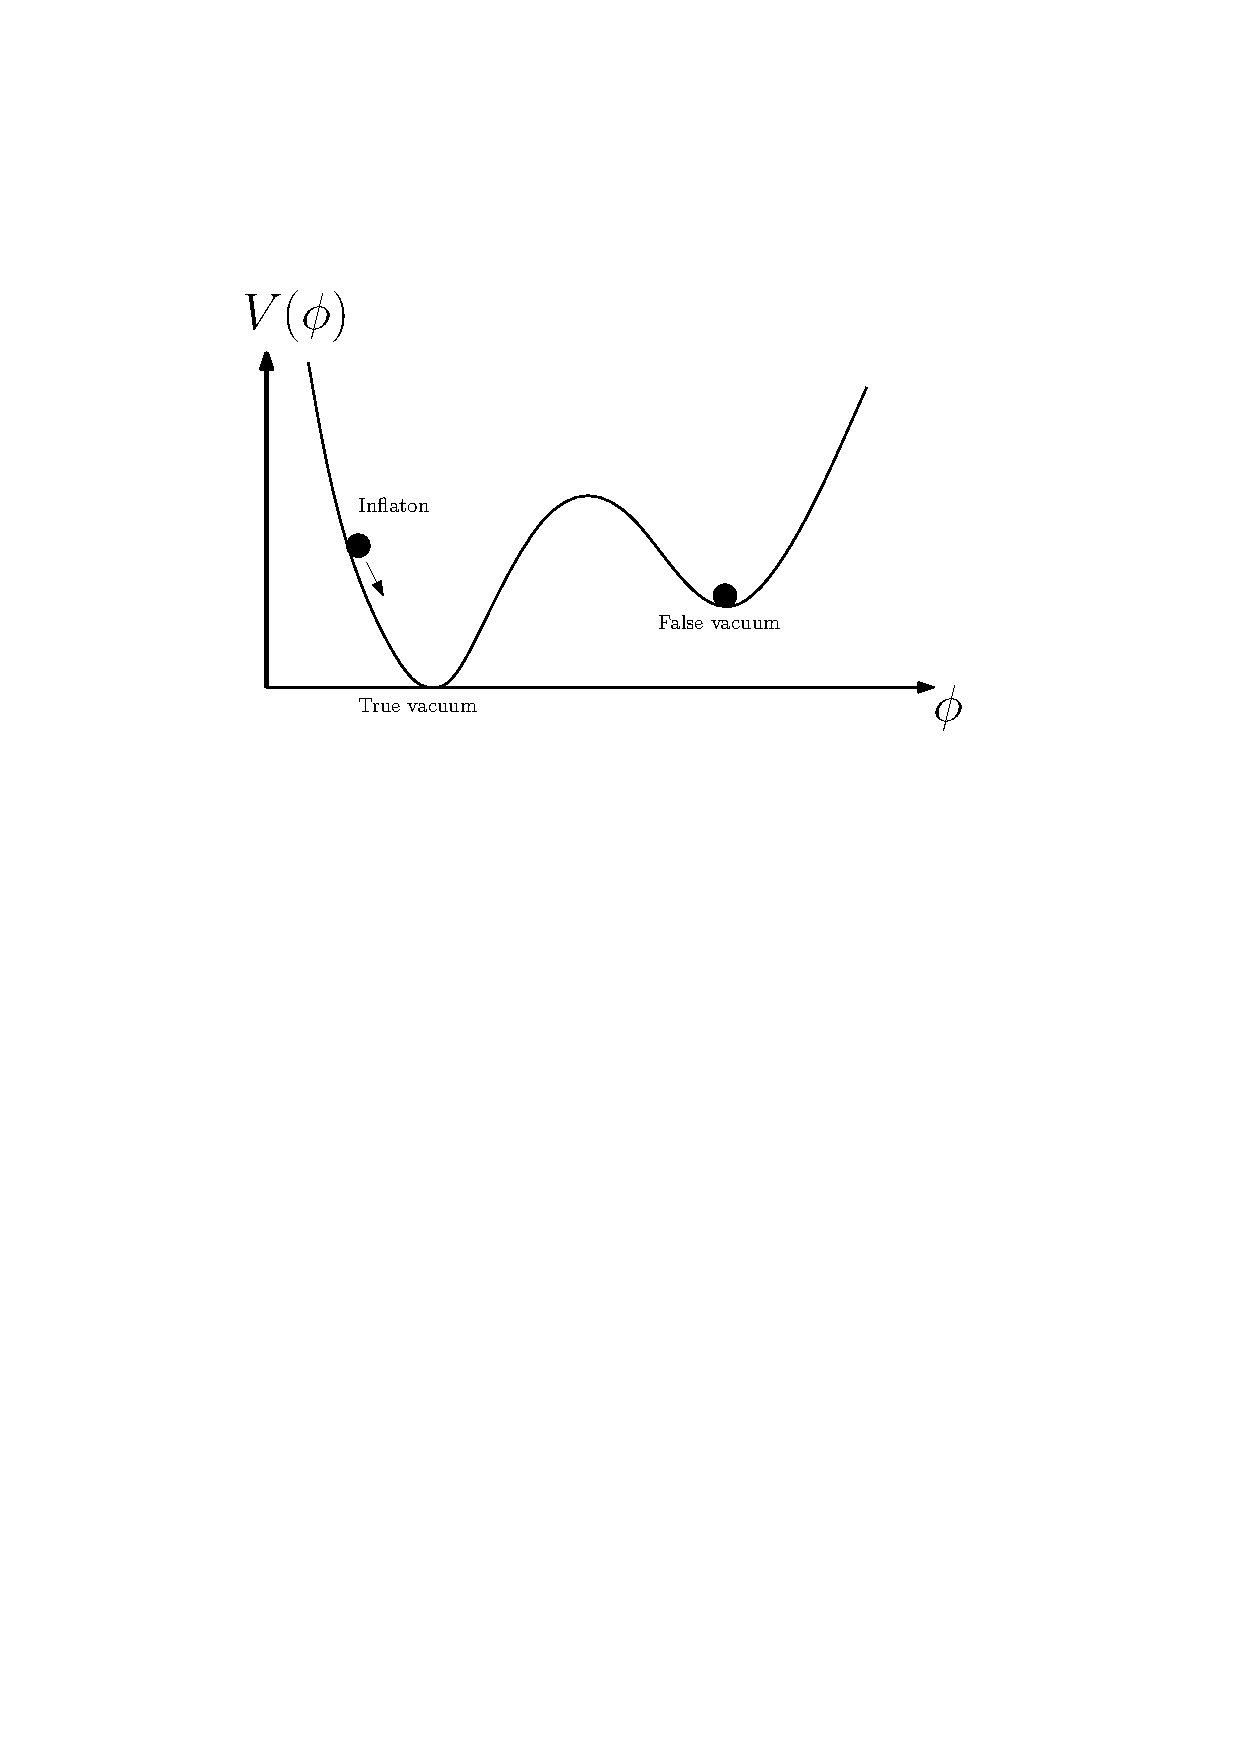
\includegraphics[width=\textwidth]{chapters/inflationary_cosmology/figures/potential}
  \caption{An example inflationary potential.}\label{fig:cos:potential}
\end{figure}

In fact, one does not need a false vacuum, one merely needs the inflaton to be rolling slowly down the potential with its speed small in comparison to the potential energy:
\begin{equation}
  \dot{\phi}^2 \ll V(\phi).
  \label{eqn:cos:slow_roll}
\end{equation}
In this case, one still has the Hubble parameter \(H\approx H_0\) being approximately constant and therefore exponential expansion. Since the frictional term in~\eqref{eqn:cos:KG} robs the particle of energy, one finds that in fact these slowly rolling phases are generic attractors for most inflationary potentials. All one requires is that the inflaton begins a reasonable way from the potential minimum.

Thus, a very general scalar particle is capable of triggering a generic exponential accelerated expansion. This epoch of the universe is termed inflation, and the particle of the field \(\phi\) the inflaton.

\subsection{Reheating}
Inflation finishes when the inflaton reaches its true vacuum, and oscillates about its minimum. One then imagines that the inflaton then decays into more traditional matter in a period called reheating. This is theoretically interesting and an area of active research. As we shall see however, for the purposes of setting initial conditions on the remainder of the contents of the universe, reheating can often be ignored.




\section{The perturbed universe}
Observationally, the real universe is not perfectly smooth.\footnote{For example, the fact that you are reading this thesis indicates that there must be some departure from homogeneity.}
We may treat the smooth FRW metric as a 0\textsuperscript{th} order approximation, to the universe, and expand about this solution using perturbation theory. In general then, we write each quantity as:
\begin{equation}
  X(t,\vx) \rightarrow X(t) + \delta X(t,\vx),
  \label{eqn:cos:expansion}
\end{equation}
where ``\(\rightarrow\)'' in this context should be read as ``is perturbed as''.
Since in the early universe the perturbations were small \(\delta X \ll X\), we may expand all equations to linear order with very high accuracy. One cannot hope to cover the full subtlety of cosmological perturbation theory in a short introductory chapter. For more detail, I highly recommend the expositions by~\cite{mukhanov_theory_1992} and~\cite{Baumann+2009}. We shall work with the perturbations to the flat FRW metric, but the analysis can be extended to the open and closed cases as well.



\subsection{Metric perturbation}
A general perturbation of the flat FRW metric will take the form:
\begin{equation}
  \d{s}^2 = (1+2\Phi)\d{t}^2 -2a B_i \d{x}^i \d{t}  -a^2 \left[ \left( 1 - 2 \Psi \right)\delta_{ij} + 2E_{ij} \right] \d{x}^i \d{x}^j,
  \label{eqn:cos:FRW_perturb}
\end{equation}
where the various terms in the above expression are defined in Table~\ref{tab:cos:perturbed_metric}, and \({\Phi,B_i,\Psi,E_{ij}\ll1}\) are small, and the tensor \(E_{ij}\) is symmetric and traceless
\begin{table}[tp]
  \centering
  
\begin{tabular}{lll}
 \toprule
  Symbol & Definition \\
 \midrule
 \midrule
 \(\Phi\) & lapse \\
 \(B_i\) & shift \\
 \(\Psi\) & (spatial) curvature perturbation  \\
 \(E_{ij}\) & (spatial) shear (3-tensor) \\
 \bottomrule
\end{tabular}

  \caption{Definitions of terms in the perturbed FRW metric. Although \(E_{ij}\) is termed the shear tensor, it is in fact its time derivative \(\dot{E}_{ij}\) which determines the shear of the worldlines of constant coordinate position.}\label{tab:cos:perturbed_metric}
\end{table}

In order to arrive at~\eqref{eqn:cos:FRW_perturb}, begin by considering a perturbation to the FRW metric tensor~\eqref{eqn:cos:FRW_metric}: \({g_{\mu\nu} \rightarrow g_{\mu\nu} + \delta g_{\mu\nu}}\). Since the background form is split into spatial and temporal parts, one may split the perturbed metric into \(\d{t}^2\), \(\d{t}\d{x^i}\) and \(\d{x^i}\d{x^j}\) terms. We may choose to define \({\delta g_{00} = 2\Phi}\), \({\delta g_{0i} = \delta g_{i0} = -a B_i}\), \({\delta g_{ij} = -2a^2F_{ij}}\). The factors of two and \(a\) are introduced for later notational convenience, and \({F_{ij} = F_{ji}}\) is symmetric. Finally, we split \({F_{ij} = -\Psi\delta_{ij} + E_{ij}}\) into a symmetric, traceless tensor \(E_{ij}\) and a scalar \(\Psi\). Putting this all together, one arrives at~\eqref{eqn:cos:FRW_perturb} above.

\subsection{Matter perturbation}
Perturbations of the matter content will take the form:
\begin{align}
  \rho \rightarrow \rho + \delta \rho, \qquad 
  P \rightarrow P + \delta P, \qquad
  u_\mu \rightarrow \left[ 1+\Phi, \delta q_i/(\rho+P)\right].
  \label{eqn:cos:matter_perturb}
\end{align}
The density and pressure perturbations are self-explanatory. The perturbation to the fluid velocity is first chosen so that \(u^\mu u_\mu=1\) to first order, and \(\delta q_i\) is the perturbation to the momentum density. The advantage of this is that for non-interacting fluids, \(\delta\rho\), \(\delta P\) and \(\delta q_i\) are all additive, as in equation~\eqref{eqn:cos:multi_component}. We have neglected a perturbation to the anisotropic stress. Anisotropic stress may be included if desired (for example in the case of neutrinos) but will add complexity unnecessary for this exposition. 

At some point one must also assume an equation of state for the fluid which provides equations to constrain \(P\) and \(\rho\). One can remain general by splitting the pressure perturbation into adiabatic and entropic parts:
\begin{equation}
  \delta P = \delta P_\mathrm{ad} + \delta P_\mathrm{en},
  \label{eqn:cos:adiabatic_entropic}
\end{equation} 
where:
\begin{equation}
  \frac{\delta P_\mathrm{ad}}{\dot{P}} = \frac{\delta\rho}{\dot{\rho}}.
  \label{eqn:cos:adiabatic}
\end{equation} 
For more detail, see~\citet[p.~48]{Baumann+2009}. 
In most cases, we limit ourselves to adiabatic matter \(\delta P_\mathrm{en}=0\).
This is not particularly restrictive, and is naturally satisfied by the equations of state~\eqref{eqn:cos:multi_component}, although it is not in general satisfied by the pressure perturbations generated by scalar fields.

The scalar field perturbation is similarly simple:
\begin{equation}
  \phi \rightarrow \phi + \delta\phi.
\end{equation}

\subsection{Fourier modes and scalar-vector-tensor decomposition}
In general, the Einstein equations~\eqref{eqn:cos:einstein_tensor} are non-linear, second order, partial differential equations and are therefore extremely challenging to solve. Perturbing about a background as in the previous section yields linearised versions of the Einstein~\eqref{eqn:cos:einsteins_equations} and conservation equations~\eqref{eqn:cos:SET_conservation}:
\begin{align}
  \delta G_{\mu\nu} &= \frac{1}{\m^2}\delta T_{\mu\nu},
  \label{eqn:cos:einsteins_equations_perturb} \\
  \delta (\nabla_\mu T^{\mu}_{\nu}) &=0,
  \label{eqn:cos:SET_conservation_perturb}
\end{align}
which greatly simplifies the analysis.  
We may go further and exploit the symmetries of the background unperturbed universe to make life even easier.

First, a general field \(\varphi(t,\vx)\) can be written in Fourier modes as:
\begin{align}
  \varphi(t,\vk) &= \int \d[3]{\vx}\: \varphi(t,\vx) e^{-i\vk \cdot \vx},\\
  \varphi(t,\vx) &= \int \frac{\d[3]{\vk}}{{(2\pi)}^3}\: \varphi(t,\vk) e^{i\vk \cdot \vx}.
\end{align}
The translational invariance of the unperturbed universe means that the Fourier modes of the perturbations decouple, turning spatial derivatives into multiples of wavevectors. 
It is worth remarking that the above decomposition is specifically for a flat universe. There are analogous approaches for the open and closed cases, but for simplicity we shall keep to the flat case. 

Second, a general spatial vector field \(v_i\) and a symmetric tensor field \(T_{ij}\) can be decomposed into helicity modes as:
\begin{align}
  v_i \rightsquigarrow& \partial_i v + v_i,   \nonumber\\
  &(\partial^k v_k=0), \\
  T_{ij} \rightsquigarrow& (\partial_i\partial_j - \frac{\delta_{ij}}{3}\partial^k\partial_k)T + \frac{1}{2}(\partial_i T_j + \partial_j T_i) + T_{ij} \nonumber,\\ 
  &(\partial^k T_k = \partial^k T_{ki} = T^k_k = 0),
\end{align}
where ``\(\rightsquigarrow\)'' in this context should be read as ``is decomposed as''.
Thus \(v\) and \(T\) are helicity scalars, \(v_i\) and \(T_i\) are divergenceless 3-vectors and \(T_{ij}\) is a divergenceless, symmetric, traceless 3-tensor\footnote{Note the overloading: \(v\) and \(T\) have different meanings on either side of each relation.}.
  The rotational invariance of the unperturbed universe means that the spatial vector and 3-tensor perturbations also decouple.

We may therefore decompose all the perturbations into Fourier components and scalar, vector and tensor parts, decoupling the modes into three parallel analyses without spatial derivatives.

For simplicity, we shall focus on the scalar part of the analysis, since vectors generically decay under an accelerated expansion, and tensors have extremely simple dynamics. Finally, one can absorb the Laplacian term of the shear tensor \(\delta_{ij}\partial^k\partial_k E\) into the definition of the curvature perturbation \(\Psi\), and henceforth we assume that \(\nabla^2 E = 0\).

\subsection{Gauge choice}
Observant readers will have noted that there are too many perturbation variables and not enough constraints.
This lack of constraint arises from the fact that the split into background and perturbation \(X\to X+\delta X\) implied by~\eqref{eqn:cos:expansion} is more subtle than first appears. 

In addition to perturbing the dynamical variables, one can also perturb the coordinate system:
\begin{align}
  t &\rightarrow t + \delta t,
  \label{eqn:cos:gauge_t}
  \\
  x^i &\rightarrow x^i  + \delta x^i,
  \label{eqn:cos:gauge_x}
\end{align}
where in general the small perturbations \(\delta t\) and \(\delta x^i\) are functions of time and space.
For a generic scalar field \(\varphi = \varphi(t,x^i)\), this coordinate perturbation will cause an alteration of the field value:
\begin{equation}
  \varphi \rightarrow \varphi - \dot{\varphi}\delta t - \partial_i\varphi\delta x^i.
\end{equation}
This means that it is easy to conflate ``true'' perturbations in the variables with coordinate perturbations. In the extreme limit of no dynamical perturbation, one can see that the coordinate transformation~\eqref{eqn:cos:gauge_t}~\&~\eqref{eqn:cos:gauge_x} will in fact generate a ``false'' perturbation in \(\varphi\) of \(\delta\varphi = -\dot{\varphi}\delta t - \partial_i\varphi\delta x^i\).

Careful calculation will show that the transformation of the dynamical scalar variables under~\eqref{eqn:cos:gauge_t}~\&~\eqref{eqn:cos:gauge_x} is in fact:
\begin{align}
  \Phi &\rightarrow \Phi - \delta \dot{t}, &
  \Psi &\rightarrow \Psi +H \delta t,  \nonumber\\
  B &\rightarrow B + \delta t/a - a\delta \dot{x}, &
  E &\rightarrow E - \delta x, \nonumber\\
  \delta\rho &\rightarrow \delta\rho - \dot{\rho}\delta t, &
  \delta P &\rightarrow \delta P - \dot{P}\delta t, \nonumber\\
  \delta q &\rightarrow \delta q + (\rho+P)\delta t,&
  \delta \phi &\rightarrow \delta \phi - \dot{\phi}\delta t,
\end{align}
where \(E\) and \(B\) are the helicity scalar parts of the shear and shift, and \(\delta x\) is the scalar part of the spatial coordinate perturbation~\eqref{eqn:cos:gauge_x}.
By choosing an appropriate coordinate transformation, one can remove the additional dynamical variables that are unconstrained by the Einstein equations. This is typically done by setting some of the perturbation variables equal to zero. This procedure is termed a {\em gauge choice}.\footnote{\(\delta X\) is defined as the difference between the value \(X\) has in the physical (perturbed) spacetime, and the value \(X\) has in the background (unperturbed) spacetime. This can only be done if there is a prescription for identifying points between the two spacetimes, and in the language of differential geometry, this is termed a {\em gauge choice}.}
Examples of popular gauge choices can be found in Table~\ref{tab:cos:gauge_choice}.

Whilst choosing a gauge will give one a set of soluble equations, the question still remains whether the perturbations really are ``true'', or in some-way coordinate-dependent. A more robust approach proposed by~\cite{Bardeen_GI} is to avoid the issue entirely and define the gauge independent variables:
\begin{align}
  \Phi^{(B)} &=  \Phi - \dot{T}, &
  \Psi^{(B)} &=  \Psi + HT, \nonumber \\
  \delta\rho^{(B)} &= \delta\rho - \dot{\rho}T, &
  \delta P^{(B)} &= \delta P - \dot{P}T, & \nonumber\\
  \delta q^{(B)} &= \delta q - (\rho + P)T, &
  \delta \phi^{(B)} &= \delta \phi - \dot{\phi}T, 
  \label{eqn:cos:bardeen}
\end{align}
where \(T = a^2[\dot{E}-B/a]\), and the superscript \((B)\) is for ``Bardeen''. The variables in~\eqref{eqn:cos:bardeen} remain unchanged under gauge transformations, and are independent of coordinate perturbations. Any perturbation in these variables cannot be ``gauged away''. Of course, these are not unique, as any linear combination of them is also gauge-invariant, but the above set results in a reasonable basis. 

Procedurally, one of  the most powerful approaches is to choose the Newtonian gauge \({B=E=B_i=0}\). In this gauge, the Bardeen variables~\eqref{eqn:cos:bardeen} are equivalent to the Newtonian ones \(X^{(B)}=X^{(\text{Newt.})}\). At the end of the computation, we may note that any equations in \(X^{(\text{Newt.})}\) will be manifestly gauge-invariant, so we may re-promote all variables \(X^{(\text{Newt.})}\) to the gauge-invariant ones \(X^{(B)}\).


\begin{table}[tp]
  \centering
  \begin{tabular}{ll}
 \toprule
  Name & Definition \\
 \midrule
 \midrule
 Synchronous & \(\Phi=B=0\) \\
 Newtonian & \(B=E=0\) \\
 Uniform density & \(\delta\rho=0\) and e.g.\ \(E=0\) \\
 Comoving & \(\delta q = E = 0\) \\
 Comoving orthogonal & \(\delta q = B = 0\) \\
 Spatially-flat & \(\Psi=E=0\) \\
 \bottomrule
\end{tabular}

\caption{Popular gauge choices for the working with the scalar perturbation equations.}\label{tab:cos:gauge_choice}
\end{table}

\section{Comoving curvature perturbation}
\label{cos:sec:comoving_curvature_perturbation}

\subsection{Classical behaviour}
\label{sec:cos:freeze_out}
It is convenient to examine the gauge-invariant variable:
\begin{equation}
  \mathcal{R} = \Psi - \frac{H}{\rho+P}\delta q.
  \label{eqn:cos:CCP}
\end{equation}
This is termed the {\em comoving curvature perturbation}, since in the comoving gauge (\(\delta q=0\)) \(\mathcal{R}=\Psi\).
After some effort, the Einstein equations~\eqref{eqn:cos:einsteins_equations}~\&~\eqref{eqn:cos:einsteins_equations_perturb} and conservation equations~\eqref{eqn:cos:SET_conservation}~\&~\eqref{eqn:cos:SET_conservation_perturb} evaluated using the perturbed metric~\eqref{eqn:cos:FRW_perturb} and the perturbed stress energy tensor~\eqref{eqn:cos:SET_perfect_fluid}~\&~\eqref{eqn:cos:matter_perturb} yield:
\begin{equation}
  \frac{\d{\mathcal{R}}}{\d{\log a}} = 
  -\frac{k^2}{a^2}\frac{\dot{P}}{\dot{\rho}}\frac{\m^2\mathcal{R}}{(5\rho + 3P)}
  -\frac{\delta P_\mathrm{en}}{\rho+P},
\end{equation}
where for simplicity we have assumed there is no anisotropic stress. For adiabatic perturbations \(\delta P_\mathrm{en}=0\), and given that \(\rho,P\sim \m^2 H^2\), \(\dot{\rho}\sim\dot{P}\), the above equation says that: \(\frac{\d{\log \mathcal{R}}}{\d{\log a}} \sim \frac{k^2}{a^2H^2}\). As the universe inflates, \(k\ll aH\), and \(\mathcal{R}\) ``freezes out'' and becomes constant.

\subsection{Quantum behaviour}
Using the Lagrangians as defined by equations~\eqref{eqn:cos:L_grav}~\&~\eqref{eqn:cos:scalar_field_lagrangian}, we may construct the action:
\begin{equation}
  S = \int \d[4]{x}\sqrt{|g|}\mathcal{L}_G + \mathcal{L}_\phi.
\end{equation}
If we expand this action to second order in \(\mathcal{R}\), we find (after some effort):
\begin{equation}
  S^{(2)} = \int \d[4]{x}\: a^3 \frac{\dot{\phi}^2}{H^2}\left[ \mathcal{\dot{R}}^2 -a^{-2}{\left( \partial_i\mathcal{R} \right)}^2 \right].
\end{equation}
Switching to conformal time and defining:
\begin{equation}
  v = z \mathcal{R}, \qquad
  z = \frac{a \dot{\phi}}{H},
\end{equation}
the action becomes~\citep[App B]{Baumann+2009}:
\begin{equation}
  S^{(2)} = \int \d[4]{x}\: \left[ {\left( v^{\prime} \right)}^2 - {\left( \partial_i v \right)}^2 + \frac{z^{\prime\prime}}{z}v^2\right],
\end{equation}
where primes denote derivatives with respect to conformal time.

To quantise, we promote the field variable \(v\) to a quantum operator, and write it as a Fourier superposition:
\begin{equation}
  v = \int \frac{\d[3]{\vk}}{{\left( 2\pi \right)}^3}
  \left[ 
    \chi_k^{\phantom\ast}(\eta) a_\vk^{\phantom\dagger}e^{i\vk\cdot\vx} + 
    \chi_k^\ast(\eta) a_\vk^{\dagger}e^{-i\vk\cdot\vx}  
  \right],
  \label{eqn:cos:mode_func_sum}
\end{equation}
of mode functions \(v_\vk = \chi_k a_\vk\).
Requiring that the canonical commutator relation:
\begin{equation}
  [ a_{\vk^{\phantom\prime}}^{\phantom\dagger}, a_{\vk^{\prime}}^{\dagger}] = {\left( 2\pi \right)}^3\delta^{(3)}\left( \vk^{\phantom\prime}-\vk^{\prime} \right),
  \label{eqn:cos:commutator}
\end{equation}
holds true, then the wavefunction \(\chi_k(\eta)\) must satisfy:
\begin{align}
  \chi_k^{\prime\prime} + \left( k^2 - \frac{z^{\prime\prime}}{z} \right) \chi_k &=0,
  \label{eqn:cos:mode_func}
  \\
  {\chi_k^{\phantom\ast}}^{\prime} 
  {\chi_k^{\ast}}^{\phantom\prime} 
  -
  {\chi_k^{\ast}}^{\prime} 
  {\chi_k^{\phantom\ast}}^{\phantom\prime} 
  &= -i.
  \label{eqn:cos:mode_func_normalisation}
\end{align}
\subsection{de Sitter limit}
A perfectly inflating universe is a de Sitter space with:
\begin{equation}
  H=\text{const.}\Rightarrow \quad a = \frac{1}{H(\eta_\mathrm{end}-\eta)} \propto e^{Ht}, \quad -\infty<\eta<\eta_\mathrm{end}.
  \label{eqn:cos:de_sitter}
\end{equation}
As discussed in Section~\ref{sec:cos:phenomonology}, pure de Sitter space may be achieved in an inflationary scenario if \(H,\phi=\mathrm{const.}\), and is approximated under the conditions of slow roll~\eqref{eqn:cos:slow_roll}. 
Thus, in a space where \(H\) and \(\dot\phi\) are both constant, \({z^{\prime\prime}/z = a^{\prime\prime}/a = 2{(\eta_\mathrm{end}-\eta)}^{-2}}\). Taking the limit as \(\dot{\phi}\to0\) creates a pure de Sitter scenario, and the differential equation~\eqref{eqn:cos:mode_func} has the general solution:
\begin{align}
  \chi_k = &A_k \frac{1}{\sqrt{2k}}\left( 1-\frac{i}{k(\eta_\mathrm{end}-\eta)} \right)e^{-ik(\eta_\mathrm{end}-\eta)}, \nonumber\\
  + &B_k \frac{1}{\sqrt{2k}}\left( 1+\frac{i}{k(\eta_\mathrm{end}-\eta)} \right)e^{ik(\eta_\mathrm{end}-\eta)},
  \label{eqn:cos:mode_func_gs}
\end{align}
whilst the mode normalisation condition~\eqref{eqn:cos:mode_func_normalisation} is:
\begin{equation}
  |B_k|^2 - |A_k|^2 = 1.
  \label{eqn:cos:mode_func_norm_AB}
\end{equation}
The overall phase in the solution~\eqref{eqn:cos:mode_func_gs} is unimportant, so along with~\eqref{eqn:cos:mode_func_norm_AB}, there are two degrees of freedom remaining. Fixing these degrees of freedom amounts to choosing the vacuum, which is easy in de Sitter space: As \(\eta\rightarrow -\infty\), the mode equations become those of Minkowski spacetime (\(\chi_k^{\prime\prime} +k^2 \chi_k=0\)). In this case, there is a well-defined choice: \(A_k=0\), \(B_k=1\), termed Bunch-Davies initial conditions. These conditions diagonalise the Hamiltonian and select the lowest energy vacuum state,\footnote{In the general case, these statements are not equivalent.} and will be discussed in greater detail in Chapter~\ref{chp:qv}.

\subsection{Power spectra}
The two point correlation function of a general spatial field \(\varphi(\vx)\) is defined as:
\begin{equation}
  \xi_\varphi(\vr) = \mean{\varphi(\vx)\varphi(\vx + \vr)}.
\end{equation}
Taking the Fourier transform of both sides with respect to \(\vx\) and \(\vr\) yields:
\begin{equation}
  \mean{\varphi(\vk)\varphi(\vk^{\prime})} = {\left( 2\pi \right)}^3\delta^{(3)}(\vk + \vk^{\prime}) \Punnorm_\varphi(\vk),
  \label{eqn:cos:power_spectrum_definition}
\end{equation}
where the power spectrum:
\begin{equation}
  \Punnorm_{\varphi}(\vk) = \int \d[3]{r}\: \xi_\varphi(\vr)e^{-i\vk\cdot\vr},
  \label{eqn:cos:dimensionless_power_spectrum}
\end{equation}
is the Fourier transform of the two-point correlation function.

For an isotropic and homogeneous space, the quantities \(\xi_\varphi(\vr)\) and \(\Punnorm_\varphi(\vk)\) are all a function of spatial distance \({\xi(\vr) = \xi(r)}\) or wavevector magnitude \({\Punnorm_\varphi(\vk) = \Punnorm_\varphi(k)}\).
It is also conventional in this case to define a ``normalised'' power spectrum as:
\begin{equation}
  \Pnorm_\varphi(k) = \frac{k^3}{2\pi^2} \Punnorm_\varphi(k),
\end{equation}
as this has the property that:
\begin{equation}
    \int \d{(\log k)} \Pnorm_\varphi(k) = \int\frac{\d[3]{k}}{{\left( 2\pi \right)}^3}\: \Punnorm_\varphi(k) = \mean{\varphi^2(x)},
\end{equation}
i.e.\ \(\Pnorm_\varphi(k)\) may be thought of as the logarithmic spectral density of the point-wise spatial variance of the field.


\subsection{Power spectrum of comoving curvature perturbations}
To compute the power spectrum of comoving curvature perturbations \(\mathcal{R}\), one therefore needs to compute the average on the left hand side of equation~\eqref{eqn:cos:power_spectrum_definition}. The two-point spatial correlation is:
\begin{equation}
  \xi_\mathcal{R}(\eta,\vr) = \mean{\mathcal{R}(\eta,\vx+\vr)\mathcal{R}(\eta,\vx)} = z^2\mean{v(\eta,\vx+\vr)v(\eta,\vx)}.
\end{equation}
Decomposing \(v\) into Fourier modes via equation~\eqref{eqn:cos:mode_func_sum}, identifying the average \(\mean{\cdot}\) above as a quantum average \(\bracket{0}{\cdot}{0}\), and applying the usual properties of creation and annihilation operators along with the commutator relation~\eqref{eqn:cos:commutator} yields:
\begin{equation}
  \xi_\mathcal{R}(\eta,\vr) = \int \frac{\d[3]{\vk}}{{(2\pi)}^3} {\left|\frac{\chi_k}{z}\right|}^2 e^{i\vk\cdot\vr}, 
\end{equation}
which allows us to read off:
\begin{equation}
  \Punnorm_\mathcal{R}(k) = {\left|\frac{\chi_k}{z}\right|}^2.
  \label{eqn:cos:power_spectrum_evaluation}
\end{equation}
As show in Section~\ref{sec:cos:freeze_out}, the value of \(\mathcal{R}_k = \chi_k/z\) freezes out at the horizon crossing time \(t_*\) when \(k\approx a_*H_*\). Under the assumption of slow-roll inflation, one can assume that the universe was effectively de Sitter from the moment of setting the Bunch-Davies initial conditions up until horizon crossing. For pure de Sitter space~\eqref{eqn:cos:de_sitter}, as \(\eta\to\eta_\mathrm{end}\),
\begin{equation}
  |\chi_k|^2 \rightarrow 2k^3 {(\eta_\mathrm{end}-\eta)}^{-2},\qquad
  a \rightarrow H_*{(\eta_\mathrm{end}-\eta)}^{-1}.
\end{equation}
Evaluating \(z = a \dot{\phi} / H\) at horizon crossing under the above approximation and computing the dimensionless form~\eqref{eqn:cos:dimensionless_power_spectrum} of the power spectrum~\eqref{eqn:cos:power_spectrum_evaluation} yields:
\begin{equation}
  \PR(k) = \frac{H_*^2}{{(2\pi)}^2}{\left( \frac{H_*}{\dot{\phi}_*} \right)}^2.
  \label{eqn:cos:inflation_power}
\end{equation}
This therefore predicts a slowly varying power spectrum, since different \(k\) modes exit at different times, \(H_*\) and \(\dot{\phi}_*\) are \(k\)-dependent. The power spectrum is normally parameterised as:
\begin{equation}
  \PR(k) = A_s {\left( \frac{k}{k_s} \right)}^{n_s-1},
  \label{eqn:cos:lcdm_power}
\end{equation}
where \(k_s\) is some pre-defined pivot scale.
Different inflationary models predict alternative values of \(A_s\) and \(n_s\), with \(n_s\) typically less than \(1\), in contrast to the Harrison-Zel'dovich spectrum.








\section{Statistics of the CMB}
\label{cos:sec:CMB_stats}
We write a general perturbation to the temperature of the photon field of the universe as:
\begin{equation}
  T(t,\vx,\vp) = T(t)\left[ 1+\Theta(t,\vx,\vp) \right],
\end{equation}
where \(\vp\) is a unit vector denoting the direction of the incoming photons as viewed at position \(\vx\). Note that this therefore encodes the inhomogeneities and anisotropies present in the photon field by virtue of having \(\vx\) and \(\vp\) dependence respectively. We may separate the angular dependence by expanding \(\Theta\) in spherical harmonics:
\begin{align}
  \Theta(t,\vx,\vp) &= \sum_{\ell=1}^{\infty}\sum_{m=-\ell}^{\ell}a_{\ell m}(t,\vx) Y_{\ell m}(\vp),\\
  a_{\ell m}(t,\vx) &= \int \d{\Omega} Y_{\ell m}^\ast(\vp) \Theta(t,\vx,\vp).
  \label{eqn:cos:alm_integral}
\end{align}
We only observe the temperature field here (at \(\vx_0\)) and now (at \(t_0\)). By taking sufficiently many measurements in different directions of \(\vp\) of the temperature field \(\Theta\) we can compute the integral~\eqref{eqn:cos:alm_integral}, to obtain \(a_{\ell m}(t_0,\vx_0)\) up to some \(\ell_{\max{}}\).\footnote{As a rough guide, if one has \(N_\mathrm{pix}\) independent pixels, there are \({(\ell_{\max{}}+1)}^2\) different \(a_{\ell m}\)'s to measure, so \(\ell_{\max{}} \sim \sqrt{N_\mathrm{pix}}\).}

In general, theories do not predict specific values of \(a_{\ell m}\), but merely tell us about the statistical distribution from which they are drawn. At each value of \(\ell\), the \((2\ell + 1)\) observations \(\{a_{\ell m}:m=-\ell\cdots\ell\}\) are typically independent realisations of the same random variable. Their mean value is zero, but they will have some non-zero variance:
\begin{equation}
  \left\langle a_{\ell m} \right\rangle = 0, \qquad
  \left\langle a_{\ell m} a_{\ell^\prime m^\prime}^\ast\right\rangle = \delta_{\ell \ell^\prime} \delta_{m m^\prime} C_\ell.
\end{equation}
Note that the error in the sample variance obeys:
\begin{equation}
  \left( \frac{\Delta C_\ell}{C_\ell} \right) = \sqrt{\frac{2}{2\ell+1}}.
\end{equation}
This means that on larger angular scales, we have fewer \(a_{\ell m}\)'s to use to compute the sample variance, and hence have a larger sample error. This is a manifestation of {\em cosmic variance}, resulting from the fact that we only have one universe to observe. 

Computing the theoretical predictions of these \(C_\ell\)'s from a given cosmology is complicated, but amounts to an integral:
\begin{equation}
    C_\ell^{XY} = \frac{2}{\pi}\int k^2 \d{k} \: \Punnorm_\mathcal{R}(k) \Delta_{X\ell}(k)\Delta_{Y\ell}(k),
\end{equation}
where \(\Delta_{X\ell}(k)\) are transfer functions. These transfer functions are computed from line of sight integrals, requiring one to evolve the contents of the universe from the \(k\)-mode's horizon re-entry point through the hot big bang era, past the surface of last scattering at recombination and all the way to the current epoch before projecting the photon field onto the sky we see today. 
 \({X\in\left\{ T,E,B \right\}}\) labels the components of the photon field corresponding to the temperature anisotropy, and the \(E\) and \(B\) polarisation modes respectively.
Treating this calculation fully is beyond the scope of this thesis, but it suffices to say that this is now extremely well understood physics, and a full set of \(C_\ell\)'s can be computed for a given cosmology using Boltzmann codes such as \CAMB{} \citep{CAMB} in a matter of seconds.


\begin{figure}[tp]
  \centering
  \tikzsetnextfilename{transfer}
  \includegraphics[width=\textwidth]{chapters/inflationary_cosmology/plots/transfer.tikz}
  \caption{History of the early universe.}\label{fig:cos:transfer}
\end{figure}

\section{Conclusions}
We have now covered all the necessary background theory. The picture is summarised in Figure~\ref{fig:cos:transfer}. Inflation's fundamental contribution to our model of the universe is that it predicts the primordial power spectrum \(\Punnorm_\mathcal{R}(k)\) at some early time. The universe's accelerated expansion then freezes these perturbations out until much later on in cosmic history, when we understand the physics in a lot more detail. We can then use standard physics to evolve these initial conditions set by inflation to make predictions about the sky that we see today.


